% ========================================================
% 1intro.tex
% ========================================================
\section{Introduction}
\label{sec:intro}

Transit venues---airports, railway stations, and bus terminals---are among the most demanding environments for WiFi. At peak hours a single departure lounge can host hundreds of users streaming video, making calls, and uploading content over a handful of access points (APs)~\cite{kougioumtzidis2025}. Unlike enterprise offices or university campuses, transit venues have a critical feature that a network controller can exploit: a substantial fraction of the congestion is \emph{announced in advance}. Departure and arrival timetables indicate when and where passenger crowds will gather, with a temporal precision rarely available in other wireless settings. Commercial WLAN controllers, however, are largely \emph{reactive}: they detect congestion after users experience degraded service and respond with local load-balancing heuristics that ignore future schedule information~\cite{du2024}.

In this paper, we investigate how schedule information can be systematically integrated into proactive radio resource optimization. We organize the investigation around four fundamental research challenges:

\begin{enumerate}
  \item \textbf{Schedule unawareness}: conventional load predictors treat AP load as a purely historical time series and discard timetable metadata that provides crucial lead time before an impending surge~\cite{pang2024}.
  \item \textbf{Reactive radio resource control}: heuristic controllers (e.g., strongest signal first or least loaded first) and conventional deep reinforcement learning (DRL) agents trained without future look-ahead cannot pre-configure channel assignments, transmit powers, and airtime allocations before crowds physically arrive~\cite{alauthman2025}.
  \item \textbf{Multi-class QoS alignment}: traffic in transit hubs is heterogeneous: VoIP requires ultra-low latency, video demands high throughput, and best-effort traffic tolerates delay. This necessitates a hybrid, multi-objective action space (continuous transmit power, discrete channel choice, and per-class airtime budgeting) that standard continuous DRL architectures struggle to coordinate stably~\cite{yu2026}.
  \item \textbf{Decentralized learning across multi-operator administrative domains}: in large transit terminals, distinct zones often belong to different administrative operators (e.g., airport authority, airline lounges, retail tenants) who cannot pool sensitive per-user association and traffic data. Isolated per-AP learners fail to exploit broader spatial correlations, while monolithic centralized learning violates data privacy boundaries~\cite{du2024}.
\end{enumerate}

To address these challenges, we propose \textbf{STAG-FedSAC}, an integrated framework that synergistically combines: (i)~a schedule-conditioned spatio-temporal graph attention Transformer (\textbf{ST-GCAT}) that forecasts multi-horizon AP load up to 30~minutes ahead; (ii)~per-AP \textbf{Soft Actor-Critic (SAC)} agents that leverage schedule context to optimize transmit power, channel selection, and quantized 802.11e EDCA airtime quotas under a Lagrangian airtime utilization constraint; and (iii)~a two-level hierarchical federated learning protocol (\textbf{HierFed-KD}) that combines intra-zone quality-weighted model averaging with inter-zone proximal knowledge distillation over a public reference dataset, eliminating raw weight exchanges across administrative boundaries. Figure~\ref{fig:architecture} presents an architectural overview, and Section~\ref{sec:roles} details the operational roles of all entities.

\begin{figure}[htbp]
  \centering
  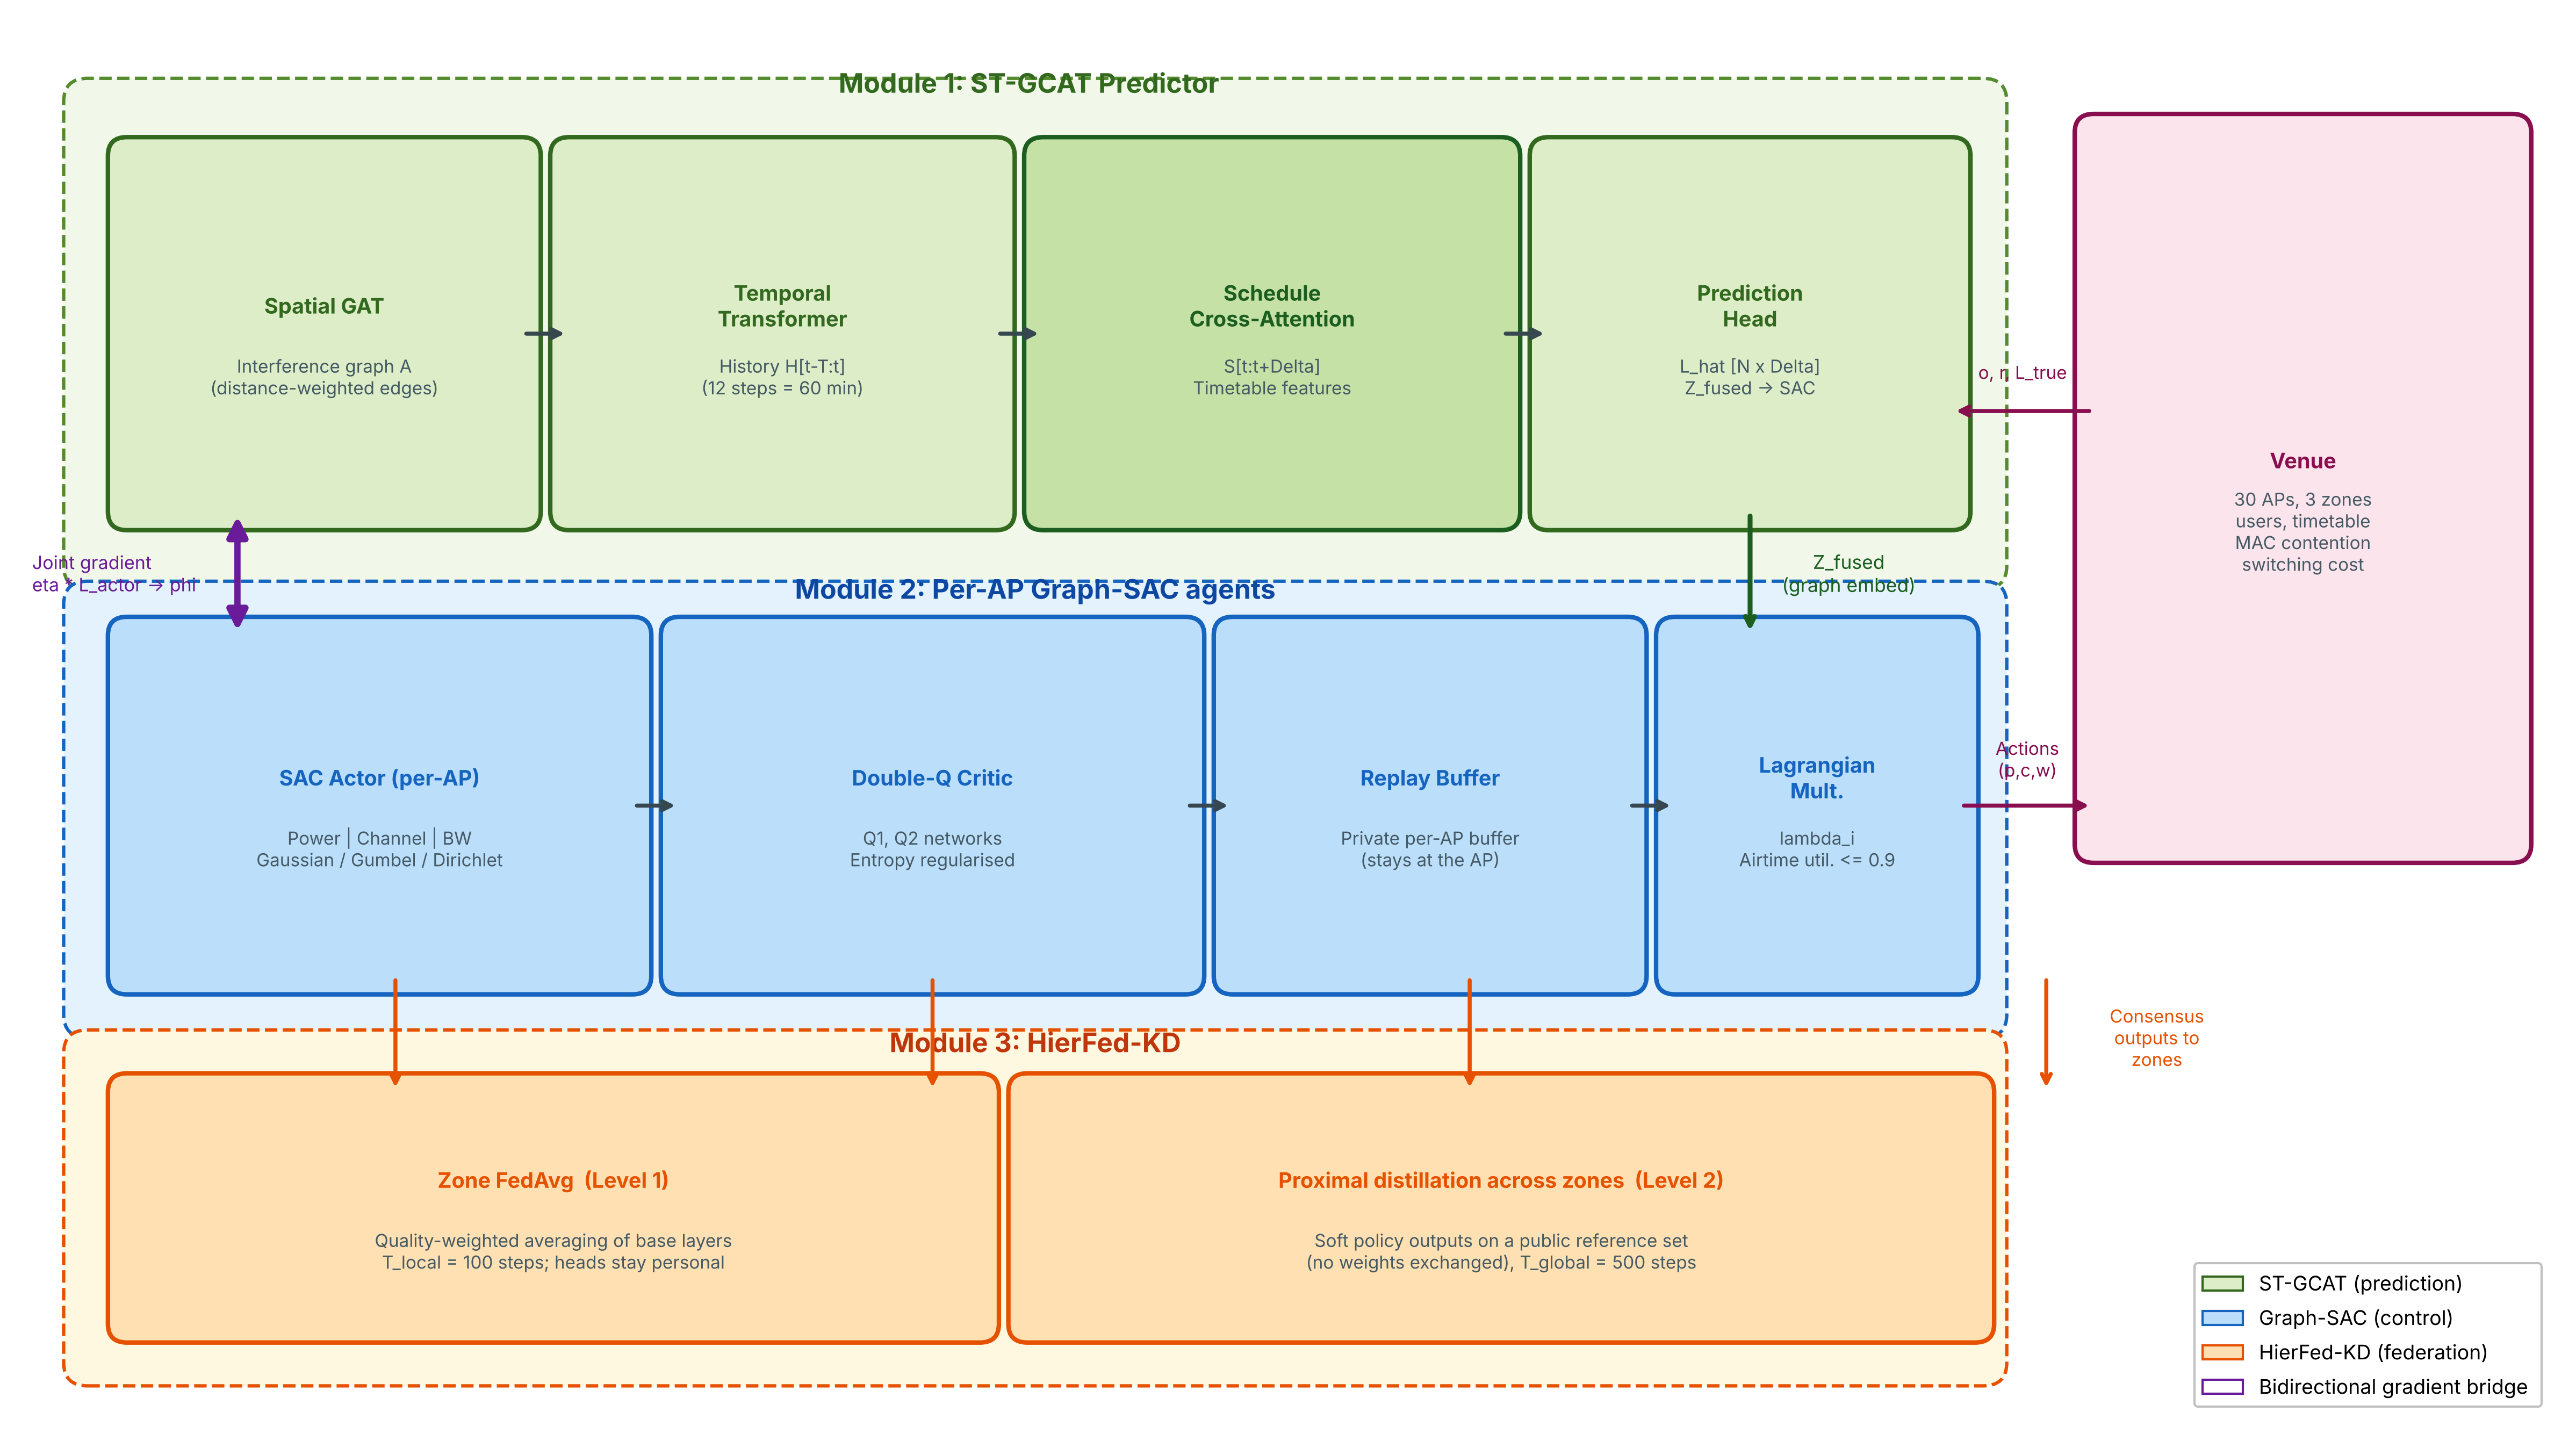
\includegraphics[width=\linewidth]{fig7_architecture.png}
  \caption{STAG-FedSAC architecture overview. Module 1 (ST-GCAT) forecasts AP load up to 30 minutes ahead from historical counters, the inter-AP interference graph, and scheduled transit timetable events, producing spatio-temporal representations. Module 2 (per-AP SAC agents) conditions on schedule context and local radio states to proactively select transmit power, channel assignment, and 802.11e EDCA airtime quotas under a Lagrangian airtime constraint. Module 3 (HierFed-KD) orchestrates two-level federation: quality-weighted parameter averaging within local zones and communication-efficient proximal distillation over a public reference set across administrative zones. Sensitive per-user association data and replay buffers remain strictly local to each AP.}
  \label{fig:architecture}
\end{figure}

\paragraph{Contributions} Our principal technical contributions are summarized as follows:
\begin{itemize}
  \item \textbf{Schedule-Conditioned Spatio-Temporal Forecasting (ST-GCAT)}: We design a cross-attention graph Transformer architecture that fuses transit timetable features (event arrival/departure times, passenger volumes, and event proximity) with historical AP counters and interference topologies, providing multi-step forecasts up to $\Delta=6$ intervals (30 minutes) ahead. ST-GCAT reduces the surge-window forecast RMSE by $39\%$ relative to persistence, by $33\%$ relative to the same predictor without the schedule and by $24\%$ relative to a temporal-only LSTM.
  \item \textbf{Proactive Multi-Objective Radio Resource Allocation}: We formulate the joint optimization of transmit power, channel selection, and multi-class QoS airtime budgeting as a constrained Markov Decision Process (CMDP). Using entropy-regularized Soft Actor-Critic with personal heads and adaptive Lagrangian multipliers, our agents reach the reward of the static incumbent plan SSF within seed variation ($\mPropReward$ against $\mSSFReward$) with a lower average user latency ($\mPropLat$~ms, $11.8\%$ below SSF at $\mSSFLat$~ms), and outperform the learned DRL baselines (FedDDPG and LSTM-DRL) by $40.5\%$--$44.7\%$ in latency and over $56\%$ in reward, with far fewer channel switches than those baselines ($0.15$ against $0.67$--$0.75$ switches/AP/step).
  \item \textbf{HierFed-KD Multi-Operator Federation}: We develop a two-level federated learning protocol that respects administrative domain boundaries. Intra-zone APs average their representations with reward-based weighting, while inter-zone coordination is achieved via proximal knowledge distillation over soft policy outputs on a public reference set. This design provides data minimisation (not a formal privacy guarantee) and reduces inter-zone wide-area communication by $\commRatioAFive\times$ relative to weight-based hierarchical federation and $\commRatioFlat\times$ relative to flat FedAvg.
  \item \textbf{Comprehensive Evaluation with Protocol Realism}: Departing from simplistic Shannon-capacity models, we implement a more realistic network simulator incorporating IEEE 802.11 MAC contention based on Bianchi's saturation model, channel-switching outage delays, and 802.11e EDCA-based airtime quotas. Multi-seed experiments (three seeds for the main comparison), paired bootstrap confidence intervals, and systematic ablation studies give insights, for our simulator, into representation design and gradient coupling for wireless reinforcement learning.
\end{itemize}

The remainder of this paper is organized as follows: Section~\ref{sec:related} surveys related work. Section~\ref{sec:method} formalizes the system model and the three modules of STAG-FedSAC. Section~\ref{sec:exp} presents experimental setup, comparative evaluations, ablation studies, and robustness analyses. Section~\ref{sec:limits} discusses deployment considerations, and Section~\ref{sec:conclusion} concludes the paper.
